\documentclass[margin=0mm]{standalone}
\usepackage[utf8]{inputenc}
\usepackage{lmodern}
\usepackage{graphics}
\usepackage{tikz,filecontents, pgfplots}
\usetikzlibrary{calc,arrows,arrows.meta,shapes,shadows,shapes.arrows,spy,angles,animations,backgrounds,decorations,patterns,babel,bending}
\usepackage{pgfplotstable}
\usepackage{siunitx}
\usepackage{gensymb}
\usepackage{amsmath}
\usepgfplotslibrary{units,fillbetween,groupplots,colorbrewer}
\usetikzlibrary{pgfplots.colorbrewer,}





%\pgfplotstableread[col sep=comma]{/media/labfiles/ruco/analisis/by-groups/pr-group/data/2021-07-26-m43140-PR-5mW.txt}\pruno
%\pgfplotstableread[col sep=comma]{/media/labfiles/ruco/analisis/by-groups/pr-group/data/2021-07-26-m43141-PR-5mW.txt}\prdos
\pgfplotstableread[col sep=comma]{/media/labfiles/ruco/analisis/by-groups/pr-group/data/2021-07-26-m43521-pr-5mW.txt}\prtres
%\pgfplotstableread[col sep=comma]{/media/labfiles/ruco/analisis/by-groups/pr-group/data/2021-07-26-m43522-PR-5mW.txt}\prcuatro
\pgfplotstableread[col sep=comma]{/media/labfiles/ruco/analisis/by-groups/pr-group/data/2021-07-26-m43523-pr-5mW.txt}\prcinco


\usepackage{relsize}
\renewcommand{\_}{\textscale{.7}{\textunderscore}}
\def\xminimo{1.50}
\def\xmaximo{1.55}
\usepackage{tikz-dimline}
\usepackage{newtxtext}
\usepackage{newtxmath}
\usepackage{scalerel}

\usepgfplotslibrary{units,fillbetween,groupplots,colorbrewer}
\usetikzlibrary{pgfplots.colorbrewer,}
\pgfplotsset{compat=newest,
	every axis/.style = {
		%scale only axis,
		width=8cm,height=5cm,
		line width = 0.7pt,
		tick style = {line width=0.7pt,black},
		ticklabel style={scale=0.8},
		major tick length = 1.5mm,
		minor tick length = 0.75mm,
		xtick pos=left,
		ytick pos=left,
		minor x tick num=1,
		minor y tick num=1,
		xlabel style={scale=0.9},
		ylabel style={scale=0.9},
		zlabel style={scale=0.9},
		xlabel={Photon energy (eV)}, 
	   	xticklabel style={
	   	/pgf/number format/precision=2,
	   	/pgf/number format/fixed,
	   	/pgf/number format/fixed zerofill,
	   },
	   yticklabel style={
	   	/pgf/number format/precision=2,
	   	/pgf/number format/fixed,
	   	/pgf/number format/fixed zerofill,
	   },
	},
	every axis plot/.style={smooth,mark=*,mark options={scale=0.5,fill=white,line width=0.5pt},line width=0.5pt},
	/pgfplots/legend image code/.code={%
		\draw[mark repeat=1,mark phase=1,#1] 
		plot coordinates {
			(0cm,0cm) 
			(0.0cm,0cm)
			(0.0cm,0cm)
			(0.0cm,0cm)
			(0.3cm,0cm)%
		};
	},
}
\pgfplotsset{every axis legend/.style={
		cells={anchor=center},
		inner xsep=1pt,
		inner ysep=1pt,
		nodes={scale=0.6,inner sep=2pt, transform shape},
		draw=none,
		at={(1,1)},
		anchor=north east,
	}
}

% \pgfplotsset{
% 	cycle from colormap manual style/.style={
% 	every axis plot/.style={smooth,mark=*,mark options={scale=0.5,fill=white,line width=0.5pt},line width=0.5pt},
% 	},
% }

% \pgfdeclareplotmark{*)}{\shade[draw=red!70!black,ball color=red!70] (0pt, 0pt) circle [radius=3pt];}
% \pgfdeclareplotmark{**)}{\shade[draw=blue!70!black,ball color=blue!70] (0pt, 0pt) circle [radius=3pt];}
% \pgfdeclareplotmark{***)}{\shade[draw=\rgb{0.31}{0.78}{0.47},ball color=\rgb{0.31}{0.78}{0.1}] (0pt, 0pt) circle
% 	[radius=3pt];}



% Commands 
% As a command
\newcommand{\m}[3]{M4\_3#1#2#3 }
\newcommand{\sm}[1]{M4\_#1}
\DeclareMathSymbol{\mh}{\mathord}{operators}{`\-}
\newcommand\thh[2]{\mathrm{e_{\scaleto{#1\mathstrut}{5pt}} \mh hh_{\scaleto{#2\mathstrut}{5pt}}}}
\newcommand\tlh[2]{\mathrm{e_{\scaleto{#1\mathstrut}{5pt}} \mh lh_{\scaleto{#2\mathstrut}{5pt}}}}
\newcommand\bandt[7]{
\path (axis cs:#1,#2) -- node[midway,scale=#6-0.1,yshift=#5,color=#7,inner sep=1pt] (point) {#4} (axis cs:#1,#3);
	\draw[-{Stealth[scale=#6]},line width=0.7pt,color=#7] (axis cs:#1,#2) -- (point) -- (axis cs:#1,#3);
}


\newcommand\trs[6]{
	\node[scale=0.8,text width = 1em,inner sep = 2pt,transform canvas={xshift=#5}] at (axis cs:#1,#2) {#6} edge [-{Stealth[scale=#4]}] (axis cs:#1,#3);
}





\pgfplotsset{every axis legend/.style={
		cells={anchor=center},
		inner xsep=1pt,
		inner ysep=1pt,
		nodes={scale=0.65,inner sep=2pt, transform shape},
		draw=none,
		at={(0,0.05)},
		anchor=south west,
	}
}


\begin{document}
	
	\begin{tikzpicture}
		\begin{axis}[
			width=10cm,height=5cm,
			name=prcomp,
			minor x tick num=1,
			ytick=\empty,
			xmin = \xminimo,xmax=\xmaximo,
			ymin=-2.5e-2,ymax=4.5e-2,
			xlabel={Photon Energy (eV)},
			ylabel={Photoreflectance},
			cycle list/Paired,
			]
			\addplot table[x index=0,y expr=\thisrowno{1}]\prtres;
			\addlegendentry{M4\_3521 n-type};
			\addplot table[x index=0,y expr=\thisrowno{1}]\prcinco;
			\addlegendentry{M4\_3523 n-type};
			
			%TRANSITIONS
			\def\sc{0.7}
			
			\bandt{1.5190}{-2e-2}{-0.75e-2}{$\thh{1}{1}$}{-3}{\sc}{Paired-A}
			\bandt{1.5212}{-2e-2}{-0.5e-2}{$\tlh{1}{1}$}{2}{\sc}{Paired-A}
			\bandt{1.5326}{-2.5e-2}{-1.6e-2}{$\thh{2}{2}$}{-3}{\sc}{Paired-A}	
			\bandt{1.5396}{-1e-2}{-0.3e-2}{$\tlh{2}{2}$}{-1}{\sc}{Paired-A}
			
			
		    \bandt{1.5286}{2.2e-2}{1.2e-2}{$\tlh{1}{2}$}{3}{\sc}{Paired-A}
			\bandt{1.5224}{1.5e-2}{0.5e-2}{$\thh{1}{2}$}{3}{\sc}{Paired-A}
			%\bandt{1.5365}{1.5e-2}{0.5e-2}{e1-lh3}{0}{\sc}{Paired-A}
		    
			\node[anchor=north west,inner sep=-0.1mm] at (axis description cs:0,1.0){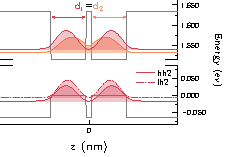
\includegraphics{/media/labfiles/ruco/analisis/by-groups/plots/cqws/build/plots-scqws.pdf}};
			
			\node[anchor=north east,inner sep=-0.1mm] at (axis description cs:1.0,1.0){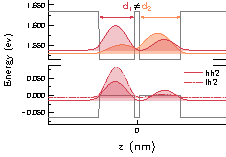
\includegraphics{/media/labfiles/ruco/analisis/by-groups/plots/cqws/build/plots-acqws-1.pdf}};
%			
%			
			\bandt{1.5300}{-1.8e-2}{-1e-2}{$\thh{1}{1}$}{-2}{\sc}{Paired-B}
			\bandt{1.5347}{-1.8e-2}{-1e-2}{$\tlh{1}{1}$}{-2}{\sc}{Paired-B}


			
			
		\end{axis}		
	\end{tikzpicture}
\end{document}
